\documentclass[serif]{beamer}\usepackage[]{graphicx}\usepackage[]{color}
%% maxwidth is the original width if it is less than linewidth
%% otherwise use linewidth (to make sure the graphics do not exceed the margin)
\makeatletter
\def\maxwidth{ %
  \ifdim\Gin@nat@width>\linewidth
    \linewidth
  \else
    \Gin@nat@width
  \fi
}
\makeatother

\definecolor{fgcolor}{rgb}{0.345, 0.345, 0.345}
\newcommand{\hlnum}[1]{\textcolor[rgb]{0.686,0.059,0.569}{#1}}%
\newcommand{\hlstr}[1]{\textcolor[rgb]{0.192,0.494,0.8}{#1}}%
\newcommand{\hlcom}[1]{\textcolor[rgb]{0.678,0.584,0.686}{\textit{#1}}}%
\newcommand{\hlopt}[1]{\textcolor[rgb]{0,0,0}{#1}}%
\newcommand{\hlstd}[1]{\textcolor[rgb]{0.345,0.345,0.345}{#1}}%
\newcommand{\hlkwa}[1]{\textcolor[rgb]{0.161,0.373,0.58}{\textbf{#1}}}%
\newcommand{\hlkwb}[1]{\textcolor[rgb]{0.69,0.353,0.396}{#1}}%
\newcommand{\hlkwc}[1]{\textcolor[rgb]{0.333,0.667,0.333}{#1}}%
\newcommand{\hlkwd}[1]{\textcolor[rgb]{0.737,0.353,0.396}{\textbf{#1}}}%
\let\hlipl\hlkwb

\usepackage{framed}
\makeatletter
\newenvironment{kframe}{%
 \def\at@end@of@kframe{}%
 \ifinner\ifhmode%
  \def\at@end@of@kframe{\end{minipage}}%
  \begin{minipage}{\columnwidth}%
 \fi\fi%
 \def\FrameCommand##1{\hskip\@totalleftmargin \hskip-\fboxsep
 \colorbox{shadecolor}{##1}\hskip-\fboxsep
     % There is no \\@totalrightmargin, so:
     \hskip-\linewidth \hskip-\@totalleftmargin \hskip\columnwidth}%
 \MakeFramed {\advance\hsize-\width
   \@totalleftmargin\z@ \linewidth\hsize
   \@setminipage}}%
 {\par\unskip\endMakeFramed%
 \at@end@of@kframe}
\makeatother

\definecolor{shadecolor}{rgb}{.97, .97, .97}
\definecolor{messagecolor}{rgb}{0, 0, 0}
\definecolor{warningcolor}{rgb}{1, 0, 1}
\definecolor{errorcolor}{rgb}{1, 0, 0}
\newenvironment{knitrout}{}{} % an empty environment to be redefined in TeX

\usepackage{alltt}
\usetheme{Boadilla}
\usepackage{graphicx}
\usepackage[final]{animate}
\usepackage{breqn}
\usepackage{xcolor}
\usepackage{booktabs}
\usepackage{tikz}
\usetikzlibrary{decorations.pathreplacing}
\usetikzlibrary{shapes,arrows,positioning,shadows}
\usepackage{subfig}
\usepackage{pgf}
\usepackage{caption}

% change format of enumerated lists
\setbeamertemplate{enumerate items}[default]
\setbeamertemplate{navigation symbols}{}

% change font size for figure captions
\setbeamerfont{caption}{size=\scriptsize}

% custom colors
\definecolor{mypal1}{HTML}{F0F9E8}\definecolor{mypal2}{HTML}{BAE4BC}\definecolor{mypal3}{HTML}{7BCCC4}\definecolor{mypal4}{HTML}{43A2CA}\definecolor{mypal5}{HTML}{0868AC}

% title graphic


\tikzstyle{decision} = [diamond, draw, text width=6em, text badly centered, inner sep = 2pt, top color=white, bottom color=mypal3, drop shadow]
\tikzstyle{block} = [rectangle, draw, text width=10em, text centered, rounded corners, minimum height=3em, minimum width=8em, top color = white, bottom color=mypal4,  drop shadow]
\tikzstyle{declare} = [rectangle, draw, text width=10em, text centered, minimum height=3em, minimum width=8em, top color = white, bottom color=mypal5,  drop shadow]

% knitr setup


% dependent data


% get online bib file


% part of figure used on title page


\setbeamercolor{title}{fg=mypal5} % main title
\setbeamercolor{frametitle}{fg=mypal4, bg=mypal2} % frame titles
\setbeamercolor{structure}{fg=mypal4} % bottom banner
\setbeamercolor{normal text}{fg=mypal5}
\usebackgroundtemplate{
\includegraphics[height=\paperheight,width=\paperwidth]{fig/back_tmp.pdf}}

% macros
\newcommand{\emtxt}[1]{\textbf{\textit{#1}}}
\IfFileExists{upquote.sty}{\usepackage{upquote}}{}
\begin{document}

\title[Seagrass light requirements]{\textbf{Quantifying seagrass light requirements using an algorithm to spatially resolve depth of colonization}}
\author[M. Beck, J. Hagy, C. Le]{Marcus W. Beck, James D. Hagy III, Chengfeng Le}

\institute[USEPA]{USEPA National Health and Environmental Effects Research Laboratory, Gulf Ecology Division, \href{mailto:beck.marcus@epa.gov}{beck.marcus@epa.gov}, Phone: 8509342480}

\date{Nov. 4, 2016}

\titlegraphic{
\begin{minipage}{0.4\textwidth}
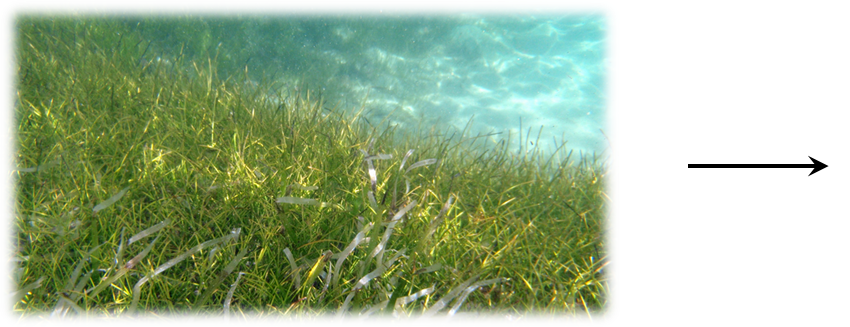
\includegraphics[width=\linewidth]{fig/titlegraphic.png}
\end{minipage}
\begin{minipage}{0.27\linewidth}
\vspace{0.05in}
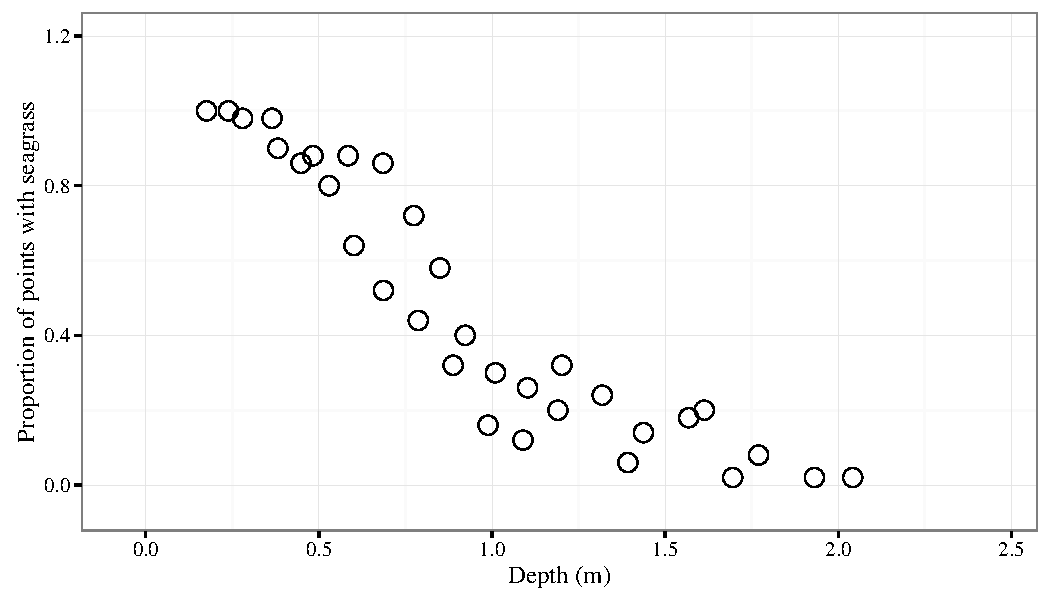
\includegraphics[width=\linewidth]{fig/doc_ex.pdf}
\end{minipage}
}

%%%%%%
\begin{frame}[shrink]
\vspace{0.2in}
\titlepage
\end{frame}

\section{Background}

%%%%%%
\begin{frame}{}

\end{frame}

%%%%%%
\begin{frame}{}

\end{frame}
% %%%%%%
% \begin{frame}{\textbf{Case 2: Seagrass and water quality}}{\textbf{Making the most of existing data}}
% \begin{center}
% Seagrass have long been considered sentinels of water quality \\~\\
% \centerline{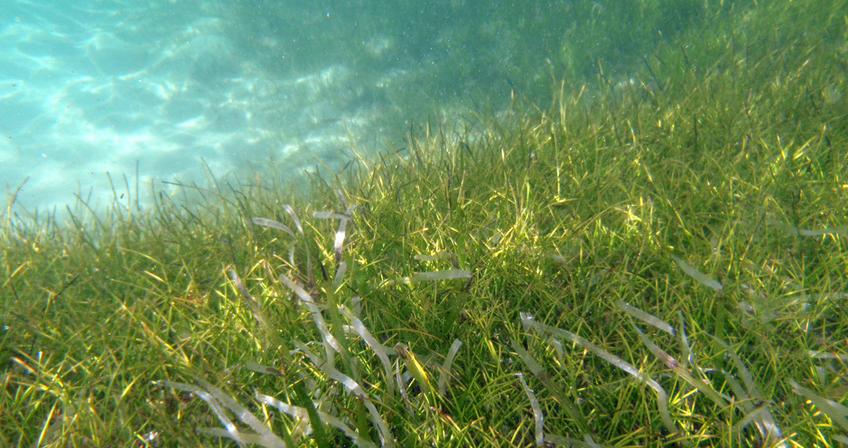
\includegraphics[width = 0.7\textwidth]{fig/sg_pic.png}}
% \vspace{0.1in}
% Seagrass provide numerous benefits - healthy seagrass, healthy estuary
% \end{center}
% \vfill
% \tiny
% \hfill \href{https://www.flickr.com/photos/swimvixen2/3581613875/in/photostream/}{flickr.com/photos/swimvixen2}
% \end{frame}
% 
% %%%%%%
% \begin{frame}{\textbf{Case 2: Seagrass and water quality}}{\textbf{Making the most of existing data}}
% \onslide<+->
% The maximum depth of colonization is a useful proxy for trophic state \\~\\
% Often used as a basis for establishing nutrient criteria \\~\\
% \onslide<+->
% \alert{Problem 1:} No consensus on the best way to measure depth of colonization\\~\\
% \alert{Problem 2:} Plenty of data are available but standardized techniques have not been developed
% \end{frame}
% 
% %%%%%%
% \begin{frame}{\textbf{Case 2: Seagrass and water quality}}{\textbf{Making the most of existing data}}
% \onslide<+->
% \alert{Solution 1:} Develop a reproducible and empirical method for estimating depth of colonization \scriptsize [Hagy et al., in prep]
% \begin{columns}[T]
% \begin{column}{0.5\textwidth}
% <</segmap, fig.height = 4, fig.width = 4, echo = F, results = 'hold', cache = T>>=
% segs <- readShapeSpatial('data/segs.shp')
% state <- readShapeSpatial('data/FL_state.shp')
% 
% par(mar = c(0, 0, 2, 0), family = 'serif')
% sp::plot(state, col = pal(5)[3])
% sp::plot(segs, col = pal(5)[2], add = T)
% title('Segment-based approach', line = 0, cex.main = 1.4)
% @
% \end{column}
% \begin{column}{0.45\textwidth}
% \centerline{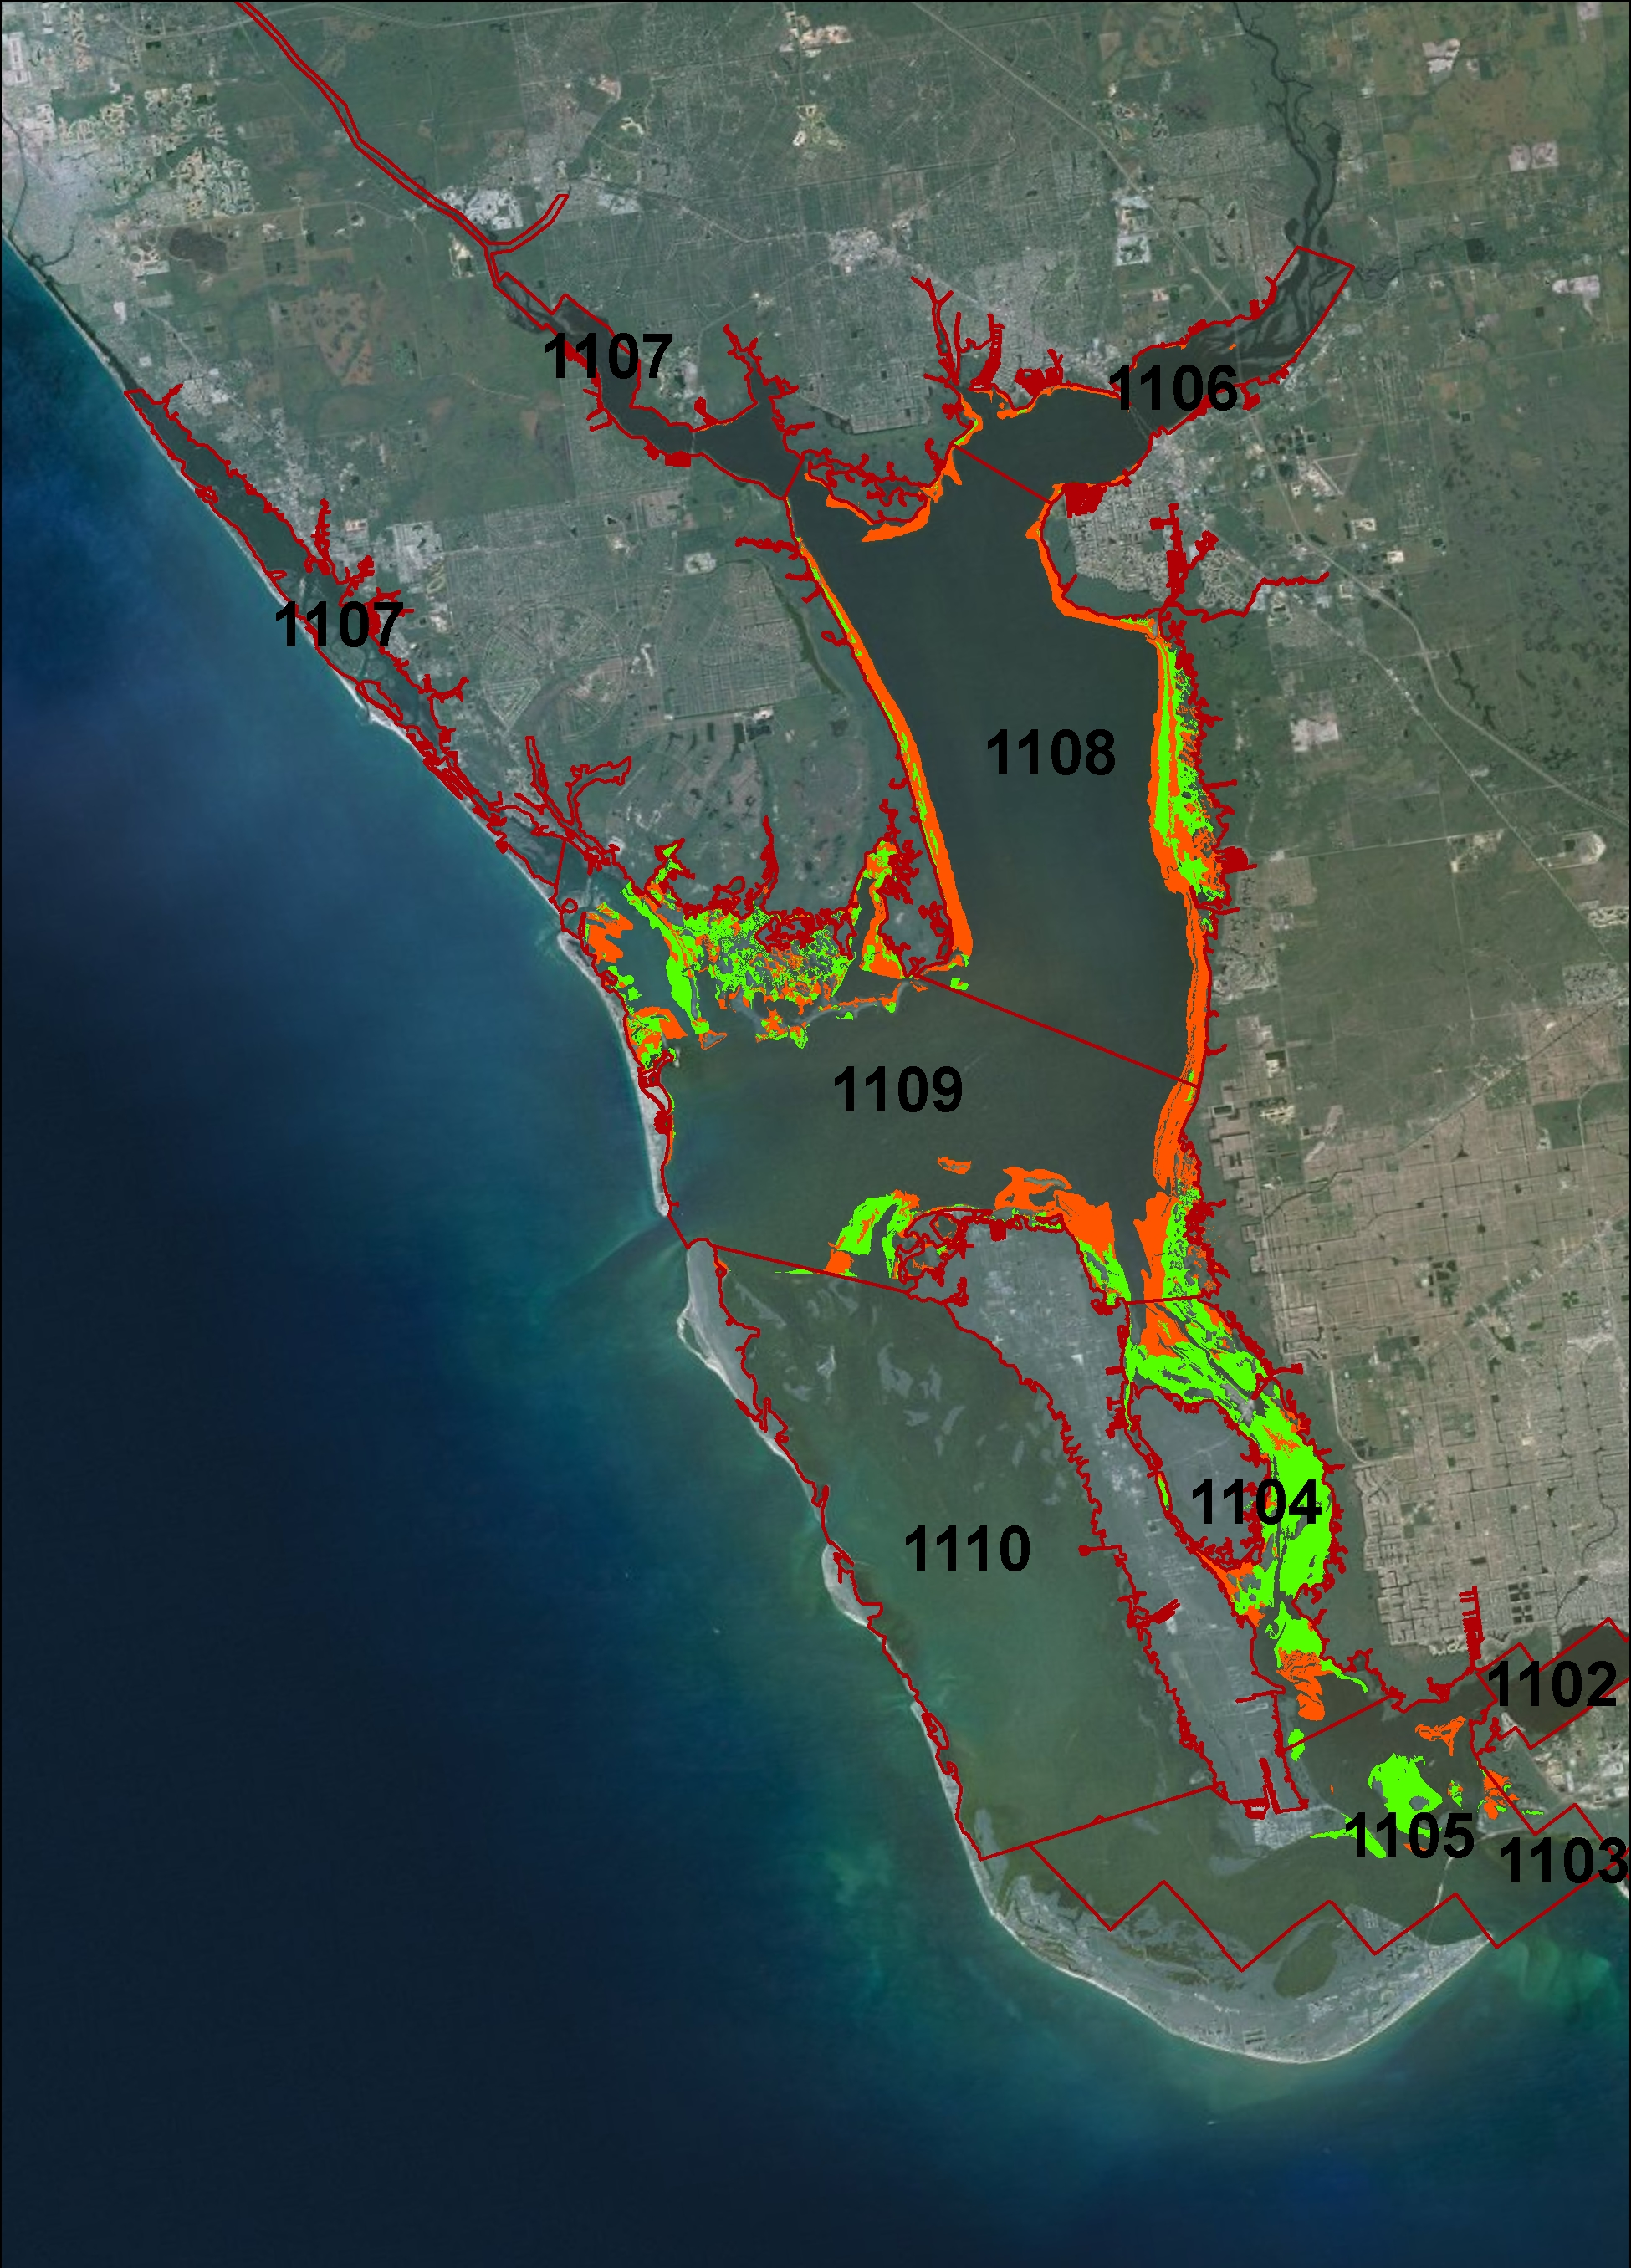
\includegraphics[width = 0.8\textwidth]{fig/Charlotte_Estuary_Segments.jpg}}
% \end{column}
% \end{columns}
% \end{frame}
% 
% %%%%%%
% \begin{frame}{\textbf{Case 2: Seagrass and water quality}}{\textbf{Making the most of existing data}}
% \onslide<+->
% How can we estimate depth of colonization? \\~\\
% \begin{columns}[T]
% \onslide<+->
% \begin{column}{0.32\textwidth}
% Pick a segment\\~\\
% \centerline{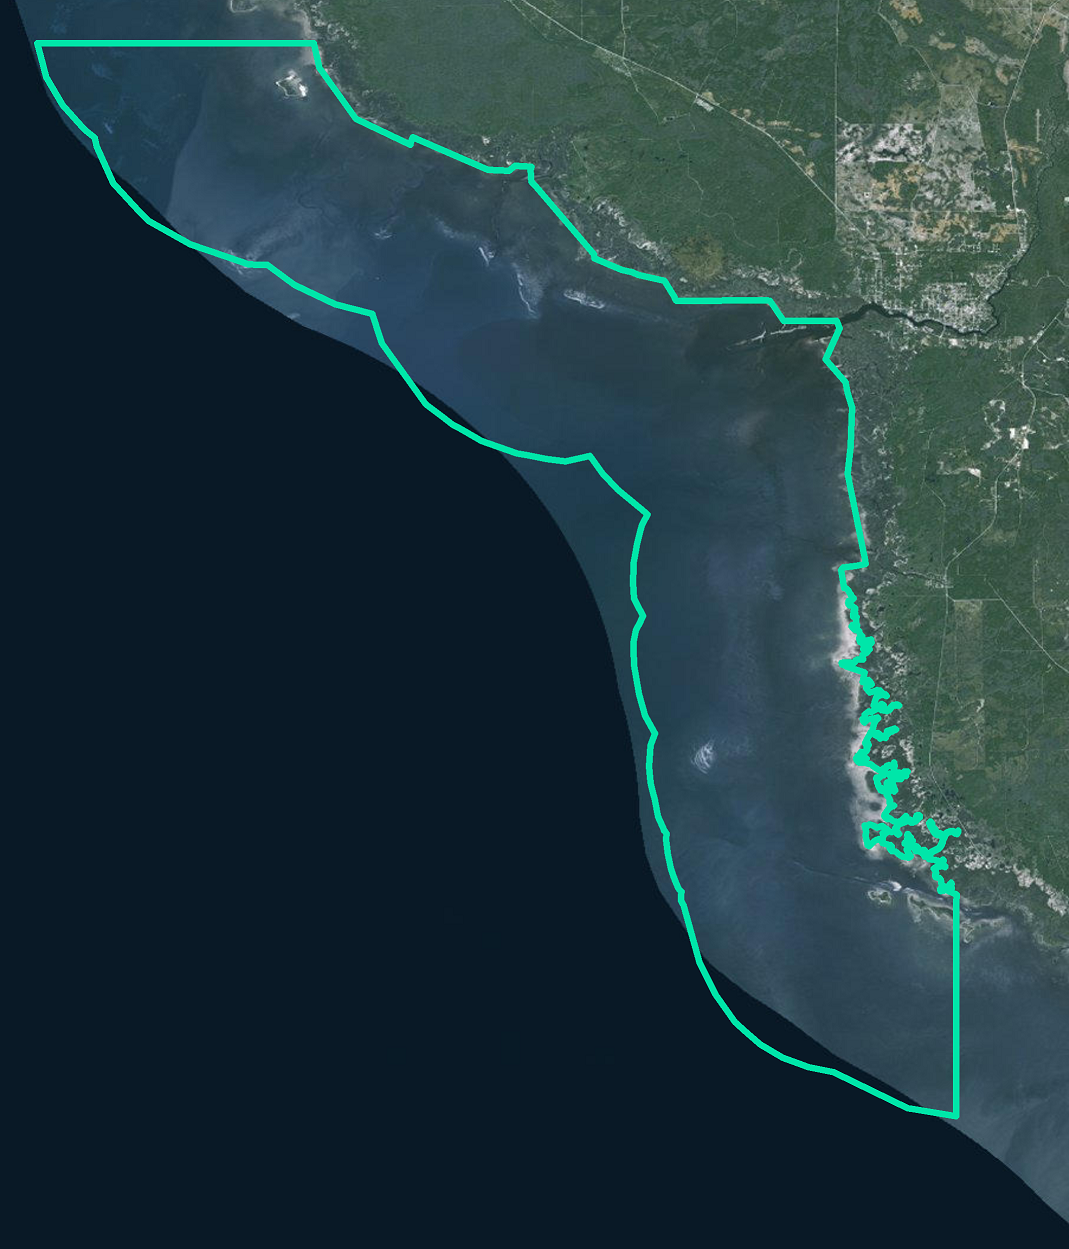
\includegraphics[width = 0.9\textwidth]{fig/map820.png}}
% \end{column}
% \onslide<+->
% \begin{column}{0.32\textwidth}
% Get seagrass coverage
% <</segsg, fig.height = 4, fig.width = 4, echo = F, results = 'hold', cache = T>>=
% seg <- readShapeSpatial('data/seg_820.shp')
% state <- readShapeSpatial('data/FL_state.shp')
% sgpoly <- readShapeSpatial('data/bbend_sg_diss.shp')
% 
% par(mar=c(0,0,0,0))
% sp::plot(seg, border = 'white')
% sp::plot(sgpoly, add = T, col = pal(5)[1], border = NA)
% sp::plot(state, add = T, col = pal(5)[3])
% sp::plot(seg, add = T)
% @
% \end{column}
% \onslide<+->
% \begin{column}{0.32\textwidth}
% Get depth points\\~\\
% <</segpt, fig.height = 4, fig.width = 4, echo = F, results = 'hold', cache = T>>=
% sgrass <- readShapeSpatial('data/sgpts_820_2006.shp')
% sgrass <- sgrass[sample(1:nrow(sgrass), 2000, replace = F),]
% 
% seg <- readShapeSpatial('data/seg_820.shp')
% state <- readShapeSpatial('data/FL_state.shp')
% 
% par(mar=c(0,0,0,0))
% sp::plot(seg)
% sp::plot(state, add = T, col = pal(5)[3])
% points(sgrass, col = alpha(pal(5)[5], 0.5), pch =16, cex = 0.6)
% @
% \end{column}
% \end{columns}
% \end{frame}
% 
% %%%%%%
% \begin{frame}{\textbf{Case 2: Seagrass and water quality}}{\textbf{Making the most of existing data}}
% Plot the distribution of seagrass by increasing depth\\~\\
% \centerline{\includegraphics[width = 0.65\textwidth]{fig/Hagy_est.png}}
% \vfill
% \tiny
% \hfill [Hagy et al., in prep]
% \end{frame}
% 
% <<sgdepthall, echo = F, eval = F>>=
% # seagrass depth of col ests
% load('data/sg_dat.RData')
% sg_dat <- lapply(split(sg_dat, sg_dat$SEGID), function(x) x[nrow(x), ])
% sg_dat <- do.call('rbind', sg_dat)
% 
% # combine depth of col with segment locations
% segs <- readShapeSpatial('data/segs.shp')
% centroids <- gCentroid(segs, byid = T)
% segs$SEGID <- as.numeric(as.character(segs$SEGID))
% 
% segs <- merge(segs, sg_dat, by = 'SEGID')
% segs <- data.frame(segs, data.frame(centroids))
% segs <- na.omit(segs[, c('SEGID', 'ZcMax', 'x', 'y')])
% 
% # state
% state <- readShapeSpatial('data/FL_state.shp')
% 
% # get points/size for plots
% col.pts <- rev(pal(nrow(segs)))[rank(segs$ZcMax)]
% rsc.pts<-scales::rescale(segs$ZcMax,c(1,7))
% 
% leg.text<-round(quantile(segs$ZcMax,c(0,0.33,0.66,1)),1)
% leg.cex<-seq(0.7,5,length=4)
% leg.col<-rev(pal(4))
% 
% # plot
% pdf('fig/sgdepthall.pdf', family = 'serif', height = 7, width = 7)
% par(mar = c(0, 0, 0, 0), family = 'serif')
% 
% sp::plot(state, col = alpha(pal(5)[3], 0.5))
% points(segs$x, segs$y, pch = 21, bg = col.pts, cex = rsc.pts)
% legend(-87,28,legend=leg.text,pt.cex=leg.cex,col=alpha('black',0.75),title='Maximum seagrass depth (m)',pch=21,bty='n',cex=1.4,y.intersp=1.4,pt.bg=leg.col,x.intersp=1.3)
% dev.off()
% @
% 
% %%%%%%
% \begin{frame}{\textbf{Case 2: Seagrass and water quality}}{\textbf{Making the most of existing data}}
% We can get an estimate of seagrass depth of colonization for each segment in Florida \scriptsize [Hagy et al., in prep]
% \vspace{-0.25in}
% \centerline{\includegraphics[width = 0.55\textwidth]{fig/sgdepthall.pdf}}
% \end{frame}
% 
% %%%%%%
% \begin{frame}{\textbf{Case 2: Seagrass and water quality}}{\textbf{Making the most of existing data}}
% \onslide<+->
% This approach works if the segment is an appropriate spatial unit to characterize seagrass...
% \begin{columns}[T]
% \onslide<+->
% \begin{column}{0.45\textwidth}
% <</docfail1, fig.height = 4, fig.width = 4, echo = F, results = 'hold', cache = T>>=
% seg <- readShapeSpatial('data/seg_820.shp')
% state <- readShapeSpatial('data/FL_state.shp')
% sgrass <- readShapeSpatial('data/sgpts_820_2006.shp')
% sgrass <- sgrass[sample(1:nrow(sgrass), 2000, replace = F),]
% above <- sgrass[sgrass$GRID_CODE >= -2.619, ]
% below <- sgrass[sgrass$GRID_CODE < -2.619, ]
% 
% par(mar=c(0,0,0,0))
% sp::plot(seg, border = 'white')
% sp::plot(state, add = T, col = pal(5)[3])
% sp::plot(seg, add = T)
% points(above, col = alpha(pal(5)[5], 0.5), pch = 16, cex = 0.6)
% points(below, col = alpha('black', 0.5), pch = 21, cex = 0.6)
% legend('bottomleft', legend = c('Within max depth estimate', 'Beyond max depth estimate'), col = c(alpha(pal(5)[5], 0.5), alpha('black', 0.5)), pch = c(16, 21), border = white)
% @
% \end{column}
% \onslide<+->
% \begin{column}{0.45\textwidth}
% <</docfail2, fig.height = 4, fig.width = 4, echo = F, results = 'hold', cache = T>>=
% seg <- readShapeSpatial('data/seg_820.shp')
% state <- readShapeSpatial('data/FL_state.shp')
% sgpoly <- readShapeSpatial('data/bbend_sg_diss.shp')
% sgrass <- readShapeSpatial('data/sgpts_820_2006.shp')
% sgrass <- sgrass[sample(1:nrow(sgrass), 2000, replace = F),]
% above <- sgrass[sgrass$GRID_CODE >= -2.619, ]
% below <- sgrass[sgrass$GRID_CODE < -2.619, ]
% 
% par(mar=c(0,0,0,0))
% sp::plot(seg, border = 'white')
% sp::plot(state, add = T, col = pal(5)[3])
% sp::plot(seg, add = T)
% points(above, col = alpha(pal(5)[5], 0.5), pch = 16, cex = 0.6)
% points(below, col = alpha('black', 0.5), pch = 21, cex = 0.6)
% sp::plot(sgpoly, add = T, col = pal(5)[1], border = NA)
% legend('bottomleft', legend = 'Actual seagrass growth', fill = alpha(pal(5)[1]), border = alpha(pal(5)[1]))
% @
% \end{column}
% \end{columns}
% \end{frame}
% 
% <<radani, eval = F, echo = F>>=
% set.seed(1234)
% seg <- readShapeSpatial('data/seg_820.shp')
% state <- readShapeSpatial('data/FL_state.shp')
% sgpoly <- readShapeSpatial('data/bbend_sg_diss.shp')
% sgrass <- readShapeSpatial('data/sgpts_820_2006.shp')
% sgrass <- sgrass[sample(1:nrow(sgrass), 2000, replace = F),]
% 
% test_pt <- sgrass[sgrass$FID_1 == '138644',]
% 
% # radii to eval
% rads <- rev(seq(0.05, 0.2, length = 40))
% 
% # get doc by radius estimates for plot
% ests <- NULL
% for(rad in rads){
% 
%   buff_pts <- buff_ext(sgrass, test_pt, buff = rad)
% 
%   doc_in <- data.frame(buff_pts)
%   doc_in$GRID_CODE <- -1 * doc_in$GRID_CODE
%   doc <- doc_est(doc_in, 'GRID_CODE', 'SEAGRASS', thresh = 0.6)
%   ests <- c(ests, doc$ests)
%   
% }
% 
% pdf('fig/radred.pdf', height = 4.25, width = 9, family = 'serif')
% for(rad in rads){
% 
%   par(mfrow = c(1, 2), mar = c(4.1, 4.1, 1, 4.1), family = 'serif')
%     
%   buff_pts <- buff_ext(sgrass, test_pt, buff = rad)  
%     
%   sp::plot(seg, border = 'white')
%   sp::plot(state, add = T, col = pal(5)[3])
%   sp::plot(seg, add = T)
%   points(buff_pts, pch = 16, col = alpha('red', 0.5), cex = 0.6)
%   points(test_pt, pch = 16, col = 'black', cex = 3)
%   legend('bottomleft', legend = c('Pt of interest', 'Depth pts in buffer'), pch = c(16, 16), col = c('black', 'red'), pt.cex = c(3, 1))
%   mtext(paste0("Radius from pt: ", round(rad, 2), " (dec. deg.)"), cex = 1.45, side = 1, line = 3)
%     
%   x <- rads
%   y <- ests
%   
%   ind <- which(rad == rads)
%   if(1 + ind > length(y)) y <- ests
%   else y[(1 + ind):length(y)] <- NA
%   plot(x, y, type = 'l', xlab = 'Radius from pt (dec. deg.)', ylab = 'Colonization estimate (m)', ylim = c(1, 3), xlim = rev(range(x)), 
%     bty = 'n', cex.lab = 1.45)
% 
% }
% dev.off()
%     
% @
% %%%%%%
% \begin{frame}{\textbf{Case 2: Seagrass and water quality}}{\textbf{Making the most of existing data}}
% If segment is not appropriate, can we define a spatial boundary for estimating seagrass depth of colonization?
% \begin{center}
% \animategraphics[controls,width=0.95\linewidth]{12}{fig/radred}{}{} %frame rate is 12 per/sec
% \end{center}
% \end{frame}
% 
% <<radani2, eval = F, echo = F>>=
% set.seed(1234)
% seg <- readShapeSpatial('data/seg_820.shp')
% state <- readShapeSpatial('data/FL_state.shp')
% sgpoly <- readShapeSpatial('data/bbend_sg_diss.shp')
% # sgrass <- readShapeSpatial('data/sgpts_820_2006_buff.shp')
% # sgrass <- sgrass[sample(1:nrow(sgrass), 3000, replace = F),]
% 
% est_pts <- grid_est(seg, spacing = 0.025)
% 
% # radii to eval
% rads <- rev(seq(0.05, 0.15, length = 40))
% 
% rad_ests <- vector('list', length = length(rads))
% names(rad_ests) <- rads
% for(rad in 1){rads){
%   cat(rad, '\t')
%   ests <- NULL
%   for(est_pt in 1:nrow(data.frame(est_pts))){
%   # get doc by radius estimates for plot
%   
%     buff_pts <- buff_ext(sgrass, est_pts[est_pt, ], buff = rad)
%   
%     doc_in <- data.frame(buff_pts)
%     doc_in$GRID_CODE <- -1 * doc_in$GRID_CODE
%     doc <- doc_est(doc_in, 'GRID_CODE', 'SEAGRASS', thresh = 0.6)
%     ests <- c(ests, doc$ests)
%     
%   }
% 
% rad_ests[[as.character(rad)]] <- ests
% 
% }
% 
% set.seed(1234)
% load('data/rad_ests.RData')
% est_pts <- grid_est(seg, spacing = 0.025)
% 
% # get colors for plotting
% col_ests <- do.call('c', rad_ests)
% col_ests <- rev(pal(length(col_ests)))[rank(col_ests)]
% col_ests <- split(col_ests, rep(rads, each = length(est_pts)))
% 
% # get sizes for plotting
% rsc_ests <- do.call('c', rad_ests)
% rsc_ests <- scales::rescale(rsc_ests, c(1, 5))
% rsc_ests <- split(rsc_ests, rep(rads, each = length(est_pts)))
% 
% # legend stuff
% leg.text<-round(quantile(do.call('c', rad_ests), c(0,0.33,0.66,1), na.rm = T),1)
% leg.cex<-seq(1,5,length=4)
% leg.col<-rev(pal(4))
% 
% # radii to eval
% rads <- rev(seq(0.05, 0.15, length = 40))
% cex_rads <- seq(100, 15, length = 40)
% 
% pdf('fig/radred2.pdf', height = 4.25, width = 9, family = 'serif')
% for(rad in 1:length(rads)){
%   
%   cat(rad, '\t')
%   par(mfrow = c(1, 2), mar = c(1, 1, 1, 1), family = 'serif')
%     
%   sp::plot(seg, border = 'white')
%   sp::plot(state, add = T, col = pal(5)[3])
%   sp::plot(seg, add = T)
%   sp::plot(est_pts, add = T, pch = 16, col = 'black')
%   sp::plot(est_pts, add = T, pch = 1, col = 'black', cex = cex_rads[rad])
%   legend('bottomleft', pch = c(16, 1), pt.cex = c(1, 4), legend = c('Pt for estimate', 'Area around pt'), cex = 1.1, bty = 'n', bg = 'white', y.intersp=1.6)
%   
%   col_est <- col_ests[names(col_ests) %in% rads[rad]][[1]]
%   rsc_est <- rsc_ests[names(rsc_ests) %in% rads[rad]][[1]]
%   
%   sp::plot(seg, border = 'white')
%   sp::plot(state, add = T, col = pal(5)[3])
%   sp::plot(seg, add = T)
%   sp::plot(est_pts, add = T, pch = 16, col =col_est, cex = rsc_est)
%   legend('bottomleft', legend=leg.text,pt.cex=leg.cex,col=leg.col,title='Maximum seagrass\ndepth (m)',pch=16,bty='n',cex=1.1,y.intersp=1.6,pt.bg=leg.col,x.intersp=1.3)
%   
% }
% dev.off()
%     
% @
% %%%%%%
% \begin{frame}{\textbf{Case 2: Seagrass and water quality}}{\textbf{Making the most of existing data}}
% This can be repeated for a number of points until we get estimates that make sense
% \begin{center}
% \animategraphics[controls,width=0.95\linewidth]{12}{fig/radred2}{}{} %frame rate is 12 per/sec
% \end{center}
% \end{frame}
% 
% %%%%%%
% \begin{frame}{\textbf{Case 2: Seagrass and water quality}}{\textbf{Making the most of existing data}}
% \onslide<+->
% Benefits of the approach: \\~\\
% \begin{itemize}
% \item The spatial unit for any estimate of seagrass growth limit is problem-specific \\~\\
% \item Allows for a `compliance-point' approach (saves time/money) \\~\\
% \item Increased understanding of seagrass growth patterns - natural and anthropogenic drivers \\~\\
% \end{itemize}
% \onslide<+->
% Lots to be done...
% \end{frame}
% 
% %%%%%%
% \begin{frame}{\textbf{Case 2: Seagrass and water quality}}{\textbf{Making the most of existing data}}
% Development widget online: \href{https://beckmw.shinyapps.io/sg_depth/}{https://beckmw.shinyapps.io/sg\_depth/}
% \centerline{\includegraphics[width = 0.75\textwidth]{fig/widget.png}}
% \end{frame}
% 
% %%%%%%
% \begin{frame}
% Acknowledgments and contact info:\\~\\
% \begin{columns}
% \begin{column}{0.9\textwidth}
% {\footnotesize
% Research staff and employees at USEPA Gulf Ecology Division, San Francisco Estuary Institute \\~\\
% David Senn, Phil Bresnahan, Emily Novick, James D. Hagy III, Thomas Jabusch
% }
% \end{column}
% \end{columns}
% \vfill
% \begin{columns}
% \begin{column}{0.5\textwidth}
% \begin{center}
% 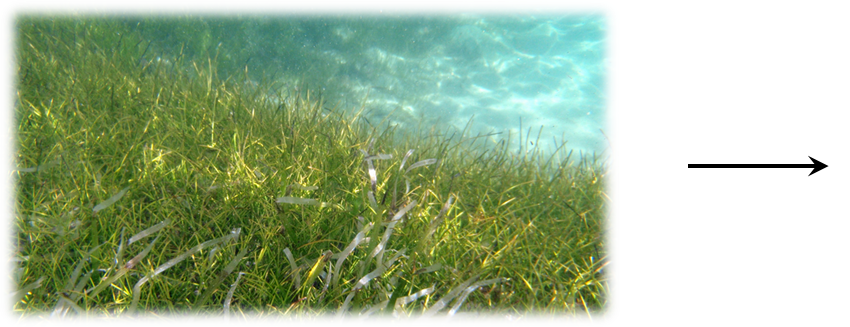
\includegraphics[width=0.7\linewidth]{fig/titlegraphic.png}
% \end{center}
% \end{column}
% \begin{column}{0.5\textwidth}
% \scriptsize
% \begin{center}
% \href{mailto:beck.marcus@epa.gov}{beck.marcus@epa.gov} \\~\\
% Github @fawda123 \\~\\
% Phone: 8509342480
% \end{center}
% \end{column}
% \end{columns}
% \vfill
% Links:\\~\\
% \begin{columns}
% \begin{column}{0.9\textwidth}
% \scriptsize
% This presentation: \href{https://github.com/fawda123/sfei_pres}{\url{https://github.com/fawda123/sfei\_pres}}
% 
% Shiny app: \href{https://beckmw.shinyapps.io/sf_trends/}{\url{https://beckmw.shinyapps.io/sf_trends/}}
% 
% Detailed results: \href{http://fawda123.github.io/sf_trends/README}{\url{http://fawda123.github.io/sf\_trends/README}}
% \end{column}
% \end{columns}
% \end{frame}

%%%%%%
\section{References}
\begin{frame}[t]{\textbf{References}}
\tiny
\setbeamertemplate{bibliography item}{}
\bibliographystyle{apalike_mine}
\bibliography{refs}
\end{frame}

\end{document}
